% To Do: Links
%        
%      
\documentclass[8pt]{extarticle}
\usepackage[english]{babel}
\usepackage[utf8]{inputenc}
\usepackage{xcolor}
\usepackage[a4paper,left=2.3cm,right=1.2cm,top=2cm,bottom=2cm]{geometry} 
\usepackage{blindtext}
\usepackage{setspace}
\usepackage{float}
\usepackage{titletoc}
\usepackage{titlesec}
\usepackage{wrapfig}
\usepackage{tikz}
\usepackage{amsmath} 
\usepackage{multicol}
\usepackage{amsfonts}
\usepackage{comment}
\usepackage{booktabs}
\usepackage{bbm}
\usepackage{wrapfig}
\usepackage{verbatimbox}
\usepackage{enumitem}
\usepackage[framemethod=TikZ]{mdframed}
\usepackage{bigints}
\onehalfspacing
\usepackage[hidelinks]{hyperref}
\usepackage[all]{nowidow} %funktioniert nicht....
\clubpenalty=9996
\widowpenalty=9999
\brokenpenalty=4991
\predisplaypenalty=10000
\postdisplaypenalty=1549
\displaywidowpenalty=1602

\setlength\parindent{0pt}



\newcommand\independent{\protect\mathpalette{\protect\independenT}{\perp}}
\def\independenT#1#2{\mathrel{\rlap{$#1#2$}\mkern2mu{#1#2}}}



%Hier sind die unterschiedlichen Ausführlichkeitsgrade definiert
\includecomment{Extensiv} 
\includecomment{Proof} 
\includecomment{Annahmen}
\includecomment{Mathspez}
\includecomment{Mathfolg}
\includecomment{Rechreg}
\mdfdefinestyle{MyFrame}{%
    linecolor=black!20!,
    outerlinewidth=0.2pt,
    roundcorner=5pt,
    innertopmargin=0.5\baselineskip,
    innerbottommargin=0.5\baselineskip,
    innerrightmargin=10pt,
    innerleftmargin=10pt,
    backgroundcolor=white}
\specialcomment{Proof}{\begin{mdframed}[style=MyFrame,nobreak=true] Proof: \ \\}{\end{mdframed}}
\specialcomment{Rechreg}{\noindent \textit{Calculation Rules:} \begin{itemize}[nosep,label=$\star$] }{\end{itemize}}
\renewcommand\ThisComment[1]{% Fix for Umlauts in comments
  \immediate\write\CommentStream{\unexpanded{#1}}%
}

% Hier die Ausführlichkeit bestimmen:
%\excludecomment{Extensiv} 
%\excludecomment{Proof} 
%\excludecomment{Annahmen}
%\excludecomment{Mathspez}
%\excludecomment{Mathfolg}

% Inhaltsverzeichnis mit zwei Spalten
\usepackage[toc]{multitoc}
\renewcommand*{\multicolumntoc}{2}




%Überschriftengrößen anpassen, so dass Paragraph kleiner ist als Subsubsection
\titleformat{\section}
  {\normalfont\fontsize{16}{15}\bfseries}{\thesection}{1em}{}
\titleformat{\subsection}
  {\normalfont\fontsize{14}{15}\bfseries}{\thesubsection}{1em}{}
\titleformat{\subsubsection}
  {\normalfont\fontsize{12}{15}\bfseries}{\thesubsubsection}{1em}{}


\begin{document}
\hrule
\begin{center}
{\fontsize{30}{60}\selectfont \textbf{Statistics}} \\ \

{\fontsize{20}{60}\selectfont Collection of Formulas}
\end{center}
\hrule
\vfill
\tableofcontents

\clearpage


% weitere Anpassungen im Hauptteil des Dokuments
\raggedright %linksbündig
\setlength{\parindent}{15pt} %Einzuglänge festsetzen
\setlength{\columnseprule}{0.3pt} %Liniendicke zwischen zwei Multicols





%-------------------------------------------------------------------------------

% SECTION: DESKRIPTIVE STATISTIK

%-------------------------------------------------------------------------------

\section{Deskriptive Statistics}


\subsection{Summary Statistics: Sample}

\begin{multicols}{2}[\subsubsection{Location}][4cm] 

\paragraph{Mode}

 Most frequent value of $x_i$. Two or more modes are possible (bimodal).

\paragraph{Median}

$$\tilde{x}_{0.5}=\begin{cases} x_{((n+1)/2)} & \text{falls }n\text{ ungerade} \\ \frac{1}{2}(x_{(n/2)}+x_{(n/2+1)} & \text{falls }n\text{ gerade} \end{cases}$$

\paragraph{Quantile}

$$\tilde{x}_\alpha=\begin{cases} x_{(k)} & \text{falls } n\alpha \notin \mathbb{N}\\ \frac{1}{2}(x_{(n\alpha)}+ x_{(n\alpha+1)}) & \text{falls } n\alpha \text{ ganzzahlig} \end{cases}$$

with

\begin{tabular}{l l}
 $k=\min x$ $\in \mathbb{N}$, &  $x$ $>$ $n\alpha$ \\
\end{tabular}

\paragraph{Minimum/Maximum}


$$x_{\min}=\min_{i \in \{ 1,...,N\}} (x_i) \hspace{0.8cm}   x_{\max}=\max_{i \in \{ 1,...,N\}} (x_i)$$
 


\paragraph{Arithmetic Mean}

 $$\bar{x}=\frac{1}{n}\sum\limits_{i=1}^n x_i$$

\noindent Estimates the expectation
$\mu = E[X]$ (first~moment).

\begin{Rechreg}
\item $E(a+b\cdot X)=a+b\cdot E(X)$
\item $E(X\pm Y)=E(X)\pm E(Y)$
\end{Rechreg}

\paragraph{Geometric Mean}

$$\bar{x}_G=\sqrt[n]{\sum\limits_{i=1}^n x_i} $$

\noindent For growth factors: $\bar{x}_G=\sqrt[n]{\frac{B_n}{B_0}}$

\paragraph{Harmonic Mean}

$$\bar{x}_H=\frac{\sum\limits_{i=1}^n w_i}{\sum\limits_{i=1}^n \frac{w_i}{x_i}}$$


\end{multicols}


\begin{multicols}{2}[\subsubsection{Dispersion}][4cm] 

\paragraph{Range}

$$R=x_{(n)}-x_{(1)}$$

\paragraph{Interquartile Range}

$$d_Q=\tilde{x}_{0.75}-\tilde{x}_{0.25}$$

\paragraph{(Empirical) Variance}

$$s^2=\frac{1}{n}\sum\limits_{i=1}^n(x_i-\bar{x})^2=\frac{1}{n}\sum\limits_{i=1}^nx_i^2-\bar{x}^2$$

\noindent Estimates the second centralized moment.

\begin{Rechreg}
\item $Var(aX+b)=a^2\cdot Var(X)$
\item $Var(X\pm Y)= Var(X)+Var(Y) + 2Cov(X,Y)$
\end{Rechreg}

\paragraph{(Empirical) Standard Deviation}

$$s=\sqrt{s^2}$$

\paragraph{Coefficient of Variation}

$$ \nu=\frac{s}{\bar{x}}$$

\paragraph{Average Absolute Deviation}


$$ \mathit{e} = \frac{1}{n}\sum_{i=1}^n \left|x_i - \bar{x}\right|$$

\noindent Estimates the first absolute centralized moment.

\end{multicols}



\begin{multicols}{2}[\subsubsection{Concentration}][4cm] 

\paragraph{Gini Coefficient}

\begin{equation*} 
\begin{split}
G & = \frac{2\sum\limits_{i=1}^n ix_{(i)}-(n+1)\sum\limits_{i=1}^n x_{(i)}}{n\sum\limits_{i=1}^n x_{(i)}}  = 1-\frac{1}{n}\sum\limits_{i=1}^n(v_{i-1}+v_i)
\end{split}
\end{equation*}

with

$$  u_i=\frac{i}{n}, \hspace{0.3cm} v_i= \frac{\sum\limits_{j=1}^i x_{(j)}}{\sum\limits_{j=1}^i x_{(j)}} \hspace{0.7cm} (u_0=0, \hspace{0.2cm} v_0=0 )$$


\noindent These are also the values for the Lorenz curve.

\ \\

\indent Range: $ 0 \le G \le \frac{n-1}{n}$




\paragraph{Lorenz-Münzner Coefficient (normed $G$)}

$$G^+=\frac{n}{n-1}G$$

\indent Range: $ 0 \le G^+ \le 1$






\end{multicols}




\begin{multicols}{2}[\subsubsection{Shape}][4cm] 

\paragraph{(Empirical) Skewness}
$$\nu = \frac{n}{(n-1)(n-2)} \sum_{i=1}^n \left(\frac{x_i-\bar{x}}{s}\right)^3$$

\noindent Estimates the third centralized moment, scaled with $(\sigma^2)^{\frac{2}{3}}$

\paragraph{(Empirical) Kurtosis}

$$k=\left[n(n+1) \cdot \sum_{i=1}^n \left(\frac{x_i-\bar{x}}{s}\right)^4 - 3(n-1)\right] \cdot \frac{n-1}{(n-2)(n-3)}+3$$

\noindent Estimates the fourth centralized moment, scaled with $(\sigma^2)^2$

\paragraph{Excess}

$$\gamma=k-3$$

\end{multicols}



\begin{multicols}{2}[\subsubsection{Dependence}][4cm]

\subsubsection*{\textit{for two nominal variables}}

\paragraph{$\chi^2$-Statistic}

\begin{equation*}
\begin{split}
\chi^2 & =\sum\limits_{i=1}^k \sum\limits_{j=1}^l \frac{(n_{ij}-\frac{n_{i+}n_{+j}}{n})^2}{\frac{n_{i+}n_{+j}}{n}}  =n\left(\sum\limits_{i=1}^k \sum\limits_{j=1}^l \frac{n_{ij}^2}{n_{i+}n_{+j}}-1\right)
\end{split}
\end{equation*}

Range: $ 0 \le \chi^2 \le n(\min(k,l)-1)$

\paragraph{Phi-Coefficient}

$$\Phi=\sqrt{\frac{\chi^2}{n}}$$

Range: $ 0 \le \Phi \le \sqrt{\min(k,l)-1}$

\paragraph{Cram\'er's $V$}

$$ V= \sqrt{\frac{\chi^2}{\min(k,l)-1}}$$

Range: $ 0 \le V \le 1$

\paragraph{Contingency Coefficient $C$}

$$C=\sqrt{\frac{\chi^2}{\chi^2 + n}}$$

Range: $ 0 \le C \le \sqrt{\frac{\min(k,l)-1}{\min(k,l)}} $

\paragraph{Corrected Contingency Coefficient $C_{corr}$}

$$C_{corr}= \sqrt{\frac{\min(k,l)}{\min(k,l)-1}} \cdot \sqrt{\frac{\chi^2}{\chi^2 + n}} $$

Range $ 0 \le C_{corr} \le 1 $

\paragraph{Odds-Ratio}

$$OR=\frac{ad}{bc} = \frac{n_{ii}n_{jj}}{n_{ij}n_{ji}}$$

Range: $0 \le OR < \infty$

\subsubsection*{\textit{for two ordinal variables}}

\paragraph{Gamma (Goodman and Kruskal)}

$$\gamma=\frac{K-D}{K+D}$$


\begin{tabular}{l l }
$ K=\sum_{i<m}\sum_{j<n}n_{ij}n_{mn}$ & Number of concordant pairs \\
$ D=\sum_{i<m}\sum_{j>n}n_{ij}n_{mn}$ & Number of reversed pairs \\
\end{tabular}

\ \\

Range: $-1 \le \gamma \le 1$

\paragraph{Kendall's $\tau_b$}

$$ \tau_b=\frac{K-D}{\sqrt{(K+D+T_X)(K+D+T_Y)}}$$

with

\begin{tabular}{l l } 
$ T_X=\sum_{i=m}\sum_{j<n}n_{ij}n_{mn}$ & Number of ties w.r.t. $X$ \\
$ T_Y=\sum_{i<m}\sum_{j=n}n_{ij}n_{mn}$ & Number of ties w.r.t. $Y$ \\
\end{tabular}

\ \\

Range: $-1 \le \tau_b \le 1$

\paragraph{Kendall's/Stuart's $\tau_c$}

$$\tau_c=\frac{2\min(k,l)(K-D)}{n^2(\min(k,l)-1)}$$

Range: $-1 \le \tau_c \le 1$

\paragraph{Spearman's Rank Correlation Coefficient}

$$\rho=\frac{n(n^2-1)-\frac{1}{2}\sum\limits_{j=1}^J b_j(b_j^2-1)-\frac{1}{2}\sum\limits_{k=1}^K c_k(c_k^2-1)-6\sum\limits_{i=1}^n d_i^2}{\sqrt{n(n^2-1)-\sum\limits_{j=1}^J b_j(b_j^2-1)}\sqrt{n(n^2-1)-\sum\limits_{k=1}^Kc_k(c_k^2-1)}}$$

or

$$\rho=\frac{s_{rg_xrg_y}}{\sqrt{s_{rg_xrg_x}s_{rg_yrg_y}}}$$

 Without ties:

$$\rho=1-\frac{6\sum\limits_{i=1}^nd_i^2}{n(n^2-1)}$$

with

\begin{tabular}{l l } 
 $d_i=R(x_i)-R(y_i)$ & rank difference \\ 
\end{tabular}

\ \\

Range: $-1 \le \rho \le 1$

\subsubsection*{\textit{for two metric variables}}

\paragraph{Correlation Coefficient (Bravais-Pearson)}

$$r=\frac{S_{xy}}{\sqrt{S_{xx}S_{yy}}}=\frac{s_{xy}}{\sqrt{s_{xx}s_{yy}}}$$

with

\begin{tabular}{l l } 
$S_{xy}=\sum\limits_{i=1}^n(x_i-\bar{x})^2(y_i-\bar{y})^2$ & or $s_{xy}=\frac{S_{xy}}{n}$ \\
$S_{xx}=\sum\limits_{i=1}^n(x_i-\bar{x})^2$ & or $s_{xx}=\frac{S_{xx}}{n}$ \\ 
$S_{yy}=\sum\limits_{i=1}^n(y_i-\bar{y})^2$ & or $s_{yy}=\frac{S_{yy}}{n}$ \\
\end{tabular}

\ \\

Range: $-1 \le r \le 1$


%\subsubsection*{\textit{Für zwei unterschiedliche Variablen}}


\end{multicols}

\subsection{Tables}

\subsection{Diagrams}

\begin{multicols}{2}[\subsubsection{Histogram}][4cm]



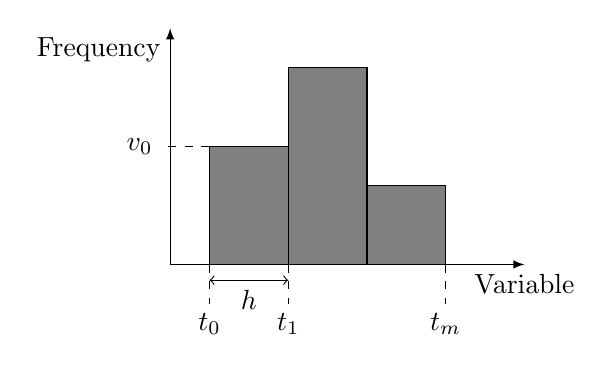
\begin{tikzpicture}

\draw[-latex] (0.5,0) -- (0.5,3) node[below left]{Frequency};
\draw[-latex] (0.5,0) -- (5,0) node[below]{Variable};

\draw[fill=black!50!] (1,0) rectangle (2,1.5);
\draw[fill=black!50!] (2,0) rectangle (3,2.5);
\draw[fill=black!50!] (3,0) rectangle (4,1);

\draw[dashed] (1,1.5) -- (0.4,1.5) node[left]{$v_0$};
\draw[dashed] (1,0) -- (1,-0.5) node[below]{$t_0$};
\draw[dashed] (2,0) -- (2,-0.5) node[below]{$t_1$};
\draw[dashed] (4,0) -- (4,-0.5) node[below]{$t_m$};
\draw[<->] (1,-0.2) -- (2,-0.2) node[midway, below]{$h$};

\end{tikzpicture}

\begin{minipage}{\columnwidth}
sample: $X=\{ x_1,x_2,...;x_n\}$ \\
$k$-th bin: $ B_k=\left[t_k,t_{k+1}\right), k=\{0,1,...,m-1\} $ \\
Number of observations in the $k$-th bin: $v_k$ \\
bin width: $h=t_{k+1}-t_k, \forall k$ \\
\end{minipage}

\paragraph{Scott's Rule}

$$h^* \approx 3.5\sigma n^{-\frac{1}{3}}$$

\noindent For approximately normal distributed data (min.\ MSE)


\end{multicols}

\subsubsection{QQ-Plot}

\subsubsection{Scatterplot}

%-------------------------------------------------------------------------------

% SECTION: PROBABILITY
%-------------------------------------------------------------------------------

\section{Probability}

\subsection{Combinatorics}

% first column
\begin{minipage}[t]{0.7\textwidth}
\addvbuffer[12pt 8pt]{\begin{tabular}{l r || c | c}
& & without replacement & with replacement \\
\midrule
Permutations & & $n!$ & $\frac{n!}{n_1!\cdot\cdot\cdot n_s!}$ \\
\midrule
Combinations: & without order & $\binom{n}{m}$ & $\binom{n+m-1}{m}$ \\
& with order & $\binom{n}{m}m!$ & $n^m$ \\
\end{tabular}}
\end{minipage}
%second column
\begin{Mathspez}
\begin{minipage}[b]{0.2\textwidth}
with: 


 $n!=n\cdot (n-1)\cdot ... \cdot 1$

 $\binom{n}{m} = \frac{n!}{m!(n-m)!}$

\end{minipage}
\end{Mathspez}


\begin{multicols}{2}[\subsection{Probability Theory}][4cm]


\paragraph{Laplace}

$$P(A)=\frac{|A|}{|\Omega|}$$


\paragraph{Kolmogorov Axioms} mathematical definition of probability

\addvbuffer[12pt 8pt]{\begin{tabular}{c l}

(1) & $0 \le P(A) \le 1 \hspace{0.5 cm} \forall A \in \mathcal{A}$ \\

(2) & $P(\Omega) = 1$ \\

(3) & $P(\bigcup_{i=1}^{\infty}{A_i}) = \sum_{i=1}^{\infty}{P(A_i)}$ \\ 
    & $\forall A_i \in \mathcal{A}, i=1,...,\infty \text{ with } A_i \cap A_j = \emptyset \text{ for } i \neq j$ \\

\end{tabular}}


\begin{Mathfolg}

Implications:
\begin{itemize}
\item $P(\bar{A})=1-P(A)$
\item $P(\emptyset)=0$
\item $P(A\cup B)=P(A)+P(B)-P(A\cap B)$
\item $A \subseteq B \Rightarrow P(A) \le P(B)$
\item $P(B)=\sum\limits_{i=1}^n P(B\cap A_i), \textnormal{ f"ur } A_i,...,A_n$  complete decomposition of $\Omega$  into pairwise disjoint events
\end{itemize}

\end{Mathfolg}

\paragraph{Probability (Mises)} frequentist definition of probability

$$P(A) = \lim\limits_{n \to \infty}\frac{n_A(n))}{n}$$

\noindent with $n$ repetitions of a random experiment and $n_A(n)$ events $A$

\paragraph{Conditional Probability}

$$P(A|B)=\frac{P(A \cap B)}{P(B)} \hspace{0.5cm} \text{für } P(B) > 0$$


$ \Rightarrow P(A \cap B)=P(B|A)P(A)=P(A|B)P(B)$

\paragraph{Law of Total Probability}

$$P(B)=\sum\limits_{i=1}^nP(B|A_i)P(A_i)$$

\paragraph{Bayes' Theorem}

$$P(A|B)=\frac{P(B|A)P(A)}{P(B)} \hspace{0.5cm} \text{for } P(A), P(B) > 0$$

\paragraph{Stochastic Independence}

\begin{alignat*}{2}
 \text{A, B independent}  \Leftrightarrow  && P(A\cap B) &= P(A)+P(B) \\
 \text{X, Y independent}  \Leftrightarrow && f_{XY}(x,y) &= f_X(x)\cdot f_Y(y) \hspace{0.5cm} \forall x,y
\end{alignat*}

\end{multicols}


\begin{multicols}{2}[\subsection{Random Variables/Vectors}][4cm]

\subsubsection*{\textit{Random Variables $\in \mathbb{R}$}}

\paragraph{Definition}

$$Y: \Omega \to \mathbb{R}$$

\noindent The Subset of possible values for $\mathbb{R}$ is called support.

\noindent Notation: Realisations of $Y$ are depicted with lower case letters. $Y=y$ means, that $y$ is the realisation of $Y$.

\paragraph{Discrete and Continuous Random Variables} \ \\

\noindent If the support is uncountably infinite, the random variable is called \textit{continuous}, otherwise it is called \textit{discrete}.

\begin{itemize}
\item \textbf{Density \boldmath$f(\cdot)$:} 

For continuous variables:
$P(Y \in \left[a, b\right]) = \int_{a}^{b} f_Y(y) dy$

For discrete variables the density (and other functions) can be depicted like the corresponding function for continuous variables, if the notation is extended as follows: 
$\int_{-\infty}^{y} f_Y(\tilde{y})d\tilde{y} := \sum_{k:k \leq y} P(Y=k)$. This notation is used.

\item \textbf{Cumulative Distribution Function \boldmath$F(\cdot)$:} 
$F_Y(y) =P(Y\leq y)$
\end{itemize}

Relationship:

$$F_Y(y) = \int_{-\infty}^{y} f_Y(\tilde{y})d\tilde{y}$$



\paragraph{Moments}

\begin{itemize}
\item \textbf{Expectation (1.\ Moment)}: $\mu = E(Y) = \int y f_Y(y)dy$
\item \textbf{Variance (2.\ centralized Moment)}: $\sigma^2 = Var(Y) = E(\{Y-E(Y)\}^2) = \int (y - E(Y))^2 f(y) dy$ \\
Note: $E(\{Y-\mu\}^2) = E(Y^2) - \mu^2$
\begin{Proof}
$E(\{Y-\mu\}^2) = E(Y^2 - 2Y\mu + \mu^2) = E(Y^2) - 2\mu^2 + \mu^2 = E(Y^2) - \mu^2$
\end{Proof}
\item \textbf{$k$th Moment}: $E(Y^k) = \int y^k f_Y(y) dy$,\\ \textbf{k.\ centralized Moment}: $E(\{Y-E(Y)\}^k)$
\end{itemize}

\paragraph{Moment Generating Function}

$$M_Y(t) = \mathrm{E}(e^{tY})$$

with $\frac{\partial^kM_Y(t)}{\partial t^k} \bigg|_{t = 0} = \mathrm{E}(Y^k)$ 

Cumulant Generating Function $K_Y(t) = \log M_Y(t)$

\noindent A random variable is uniquely defined by its moment generating function and vice versa (as long as moments and cumulants are finite).
  
\subsubsection*{\textit{Random Vectors $\in \mathbb{R}^q$}}

\paragraph{Density and Cumulative Distribution Function}

$$F(y_1, ..., y_q) = P(Y_1 \leq y_1, ..., Y_q \leq y_q)$$
\begin{align*}
& P(a_1 \leq Y_1 \leq b_1, ..., a_q \leq Y_q \leq b_q) \\
& = \int_{a_1}^{b_1} ...\int_{a_q}^{b_q} f(y_1, .., y_q)dy_1...dy_q
\end{align*}

\paragraph{Marginal Density}

$$f_{Y_1}(y_1) = \int_{-\infty}^{\infty}...\int_{-\infty}^{\infty} f(y_1,...,y_k)dy_2...dy_k$$

\paragraph{Conditional Density}

$$f_{Y_1|Y_2}(y_1|y_2) = \frac{f(y_1, ..., y_2)}{f(y_2)} \text{ for } f(y_2) > 0$$

\paragraph{Iterated Expectation}

$$\mathrm{E}(Y)=\mathrm{E}_X(\mathrm{E}(Y|X))$$
\begin{Proof}
$$\mathrm{E}(Y) = \int yf(y)dy = \int\int y f(y|x)dy f_X(x)dx = \mathrm{E}_X(\mathrm{E}(Y|X))$$
\end{Proof}
$$\mathrm{Var}(Y) = \mathrm{E}_X(\mathrm{Var}(Y|X)) + \mathrm{Var}_X(\mathrm{E}(Y|X))$$
\begin{Proof}
\begin{align*}
\mathrm{Var}(Y) =&  \int (y- \mu_Y)^2 f(y)dy\\
=& \int (y- \mu_Y)^2 f(y|x)f(x)dydx\\
=& \int (y- \mu_{Y|x} + \mu_{Y|x} - \mu_Y)^2 f(y|x)f(x)dydx\\
=& \int (y- \mu_{Y|x})^2 f(y|x)f(x)dydx + \\
 & \int (\mu_{Y|x} - \mu_Y)^2 f(y|x)f(x)dydx + \\
 & 2 \int (y- \mu_{Y|x})(\mu_{Y|x} - \mu_Y) f(y|x)f(x)dydx \\
=& \int \mathrm{Var}(Y|x)f(x)dx + \int (\mu_{Y|x} - \mu_Y)^2f(x)dx\\
=& \mathrm{E}_X(\mathrm{Var}(Y|X)) + \mathrm{Var}_X(\mathrm{E}(Y|X))
\end{align*}
\end{Proof}

\end{multicols}

\subsection{Probability Distributions}

\begin{multicols}{2}[\subsubsection{Discrete Distributions}][4cm]

  \paragraph{Discrete Uniform}
  
    \begin{align*}
    & Y \sim \mathrm{U}(\{y_1, ..., y_k\}),\: y \in \{y_1, ..., y_k\} \\
    & P(Y=y_i) =\frac{1}{k},\: i = 1, ...,k \\
    & \mathrm{E}(Y) = \frac{k+1}{2} ,\: \mathrm{Var}(Y) = \frac{k^2 - 1}{12}
  \end{align*}
  
    \paragraph{Binomial}
  Successes in independent trials 

  \begin{align*}
    & Y \sim \mathrm{Bin}(n, \pi) \text{ with } n \in \mathbb{N}, \pi \in \left[0,1\right] ,\: y \in \{0, ..., n\} \\
    & P(Y=y|\lambda) = \binom{n}{y}\pi^k(1-\pi)^{n-y} \\
    & \mathrm{E}(Y|\pi,n) = n\pi ,\: \mathrm{Var}(Y|\pi,n) = n\pi(1-\pi)
  \end{align*}

  \paragraph{Poisson}
  Counting model for rare events

\noindent only one event at a time, no autocorrelation, mean number of events over time is constant and proportional to length of the considered time interval 

  \begin{align*}
    & Y \sim \mathrm{Po}(\lambda) \text{ with } \lambda \in \left[ 0, + \infty \right] ,\: y \in \mathbb{N}_0 \\
    & P(Y=y|\lambda) =\frac{\lambda^y exp^{-\lambda}}{y!} \\
    & \mathrm{E}(Y|p) = \lambda ,\: \mathrm{Var}(Y|p) = \lambda
  \end{align*}

\noindent The model tends to overestimate the variance (Overdispersion).
  
\noindent   \textit{Approximation} of the Binomial for small p

  
    \paragraph{Geometric}

  \begin{align*}
    & Y \sim \mathrm{Geom}(\pi) \text{ with } \pi \in \left[0,1\right] ,\: y \in \mathbb{N}_0 \\
    & P(Y=y|\pi) = \pi(1-\pi)^{y-1} \\
    & \mathrm{E}(Y|\pi) = \frac{1}{\pi} ,\: \mathrm{Var}(Y|\pi) = \frac{1-\pi}{\pi^2}
  \end{align*}
  
    \paragraph{Negative Binomial}

  \begin{align*}
    & Y \sim \mathrm{NegBin}(\alpha, \beta) \text{ with } \alpha, \beta \geq 0 ,\: y \in \mathbb{N}_0 \\
    & P(Y=y|\alpha, \beta) = \binom{\alpha + y - 1}{\alpha - 1} \left(\frac{\beta}{\beta - 1}\right)^{\alpha} \left(\frac{1}{\beta + 1}\right)^y \\
    & \mathrm{E}(Y|\alpha,\beta) = \frac{\alpha}{\beta} ,\: \mathrm{Var}(Y|\alpha,\beta) = \frac{\alpha}{\beta^2}(\beta+1)
  \end{align*}

\end{multicols}

\begin{multicols}{2}[\subsubsection{Continuous Distributions}][4cm]

	\paragraph{Continuous Uniform}
  
    \begin{align*}
    & Y \sim \mathrm{U}(a,b) \text{ with } \alpha, \beta \in \mathbb{R}, a \le b,\: y \in \left[a,b\right] \\
    & p(y|a,b) =\frac{1}{b-a} \\
    & \mathrm{E}(Y|a,b) = \frac{a+b}{2} ,\: \mathrm{Var}(Y|a,b) = \frac{(b-a)^2}{12}
  \end{align*}
  
    \paragraph{Univariate Normal} symmetric with $\mu$ and $\sigma^2$
  
    \begin{align*}
    & Y \sim \mathrm{N}(\mu, \sigma^2) \text{ with } \mu \in \mathbb{R}, \sigma^2 > 0,\: y \in \mathbb{R} \\
    & p(y|\mu, \sigma^2) =\frac{1}{\sqrt{2\pi\sigma^2}} \exp \left(-\frac{(y-\mu)^2}{2 \sigma^2} \right) \\
    & \mathrm{E}(Y|\mu, \sigma^2) = \mu ,\: \mathrm{Var}(Y|\mu, \sigma^2) = \sigma^2
  \end{align*}
  
    \paragraph{Multivariate Normal} symmetric mit $\mu_i$ and $\Sigma$
  
    \begin{align*}
    & Y \sim \mathrm{N}(\mu, \Sigma) \text{ with } \mu \in \mathbb{R}^d, \Sigma \in \mathbb{R}^{d\times d} s.p.d.,\: y \in \mathbb{R}^d \\
    & p(y|\mu, \Sigma) = (2\pi)^{-\frac{d}{2}} \det (\Sigma)^{-\frac{1}{2}} \exp \left( -\frac{1}{2}(y-\mu)^{T} \Sigma^{-1}(y-\mu)\right) \\
    & \mathrm{E}(Y|\mu, \Sigma) = \mu ,\: \mathrm{Var}(Y|\mu, \Sigma) = \Sigma
  \end{align*}
  
    \paragraph{Log-Normal}
  
    \begin{align*}
    & Y \sim \mathrm{LogN}(\mu, \sigma^2) \text{ eith } \mu \in \mathbb{R}, \sigma^2 > 0,\: y > 0 \\
    & p(y|\mu, \sigma^2) =\frac{1}{\sqrt{2\pi\sigma^2 y}} \exp \left(-\frac{(\log y-\mu)^2}{2 \sigma^2} \right) \\
    & \mathrm{E}(Y|\mu, \sigma^2) = \exp (\mu + \frac{\sigma^2}{2}) ,\\
    & \mathrm{Var}(Y|\mu, \sigma^2) = \exp (2\mu + \sigma^2)(\exp (\sigma^2) - 1)
  \end{align*}
  
\noindent Relationship: $\log (Y) \sim \mathrm{N}(\mu, \sigma^2) \Rightarrow Y \sim \mathrm{LogN}(\mu, \sigma^2)$
  
    \paragraph{non-standardized Student's t} statistical Tests for $\mu$ with unknown (estimated) variance and $\nu$ degrees of freedom
  
    \begin{align*}
    & Y \sim \mathrm{t}_\nu(\mu, \sigma^2) \text{ with } \mu \in \mathbb{R}, \sigma^2, \nu > 0,\: y \in \mathbb{R}\\
    & p(y|\mu, \sigma^2, \nu) =\frac{\Gamma \left( \frac{\nu + 1}{2}\right) }{\Gamma (\frac{\nu}{2}) \Gamma (\sqrt{\nu\pi}\sigma)} \left(1+ \frac{(y-\mu)^2}{\nu \sigma^2} \right)^{-\frac{\nu + 1}{2}} \\
    & \mathrm{E}(Y|\mu, \sigma^2, \nu) = \mu \text{ for }  \nu > 1,\\
    & \mathrm{Var}(Y|\mu, \sigma^2, \nu) = \sigma^2 \frac{\nu}{\nu-2} \text{ for }  \nu > 2
  \end{align*}
  
 \noindent Relationship: $Y|\theta \sim \mathrm{N}(\mu, \frac{\sigma^2}{\theta}), \: \theta \sim  \mathrm{Ga}(\frac{\nu}{2}, \frac{\nu}{2}) \Rightarrow Y \sim \mathrm{t}_\nu(\mu, \sigma)$ 
 $t_\nu(\mu,\sigma^2)$ has heavier tails then the normal distribution. $t_\infty(\mu,\sigma^2)$ approaches $\mathrm{N}(\mu,\sigma^2)$.
  
	\paragraph{Beta}
  
    \begin{align*}
    & Y \sim \mathrm{Be}(a, b) \text{ with } a,b > 0,\: y \in \left[0,1\right]\\
    & p(y|a, b) =\frac{\Gamma \left( a+b\right) }{\Gamma (a) \Gamma (b)} y^{a-1} (1-y)^{b-1} \\
    & \mathrm{E}(Y|a, b) = \frac{a}{a+b},\\
    & \mathrm{Var}(Y|a, b) = \frac{ab}{\left(a+b\right)^2(a+b+1)}, \\
    & \mathrm{mod}(Y|a, b) = \frac{a-1}{a+b-2} \text{ f"ur } a,b > 1
  \end{align*}
  
  
  	\paragraph{Gamma}
  
    \begin{align*}
    & Y \sim \mathrm{Ga}(a, b) \text{ with } a,b > 0,\: y > 0\\
    & p(y|a, b) = \frac{ b^a }{\Gamma (a)} y^{a-1} \exp (-by) \\
    & \mathrm{E}(Y|a, b) = \frac{a}{b},\\
    & \mathrm{Var}(Y|a, b) = \frac{a}{b^a}, \\
    & \mathrm{mod}(Y|a, b) = \frac{a-1}{b} \text{ f"ur } a \ge 1
  \end{align*}

  	\paragraph{Inverse-Gamma}
  
    \begin{align*}
    & Y \sim \mathrm{IG}(a, b) \text{ with } a,b > 0,\: y > 0\\
    & p(y|a, b) = \frac{ b^a }{\Gamma (a)} y^{-a-1} \exp (-\frac{b}{y}) \\
    & \mathrm{E}(Y|a, b) = \frac{b}{a-1} \text{ f"ur } a > 1,\\
    & \mathrm{Var}(Y|a, b) = \frac{b^2}{(a-1)^2(a-2)} \text{ f"ur } a \ge 2, \\
    & \mathrm{mod}(Y|a, b) = \frac{b}{a+1}
  \end{align*}
  
\noindent Relationship: $Y^{-1} \sim \mathrm{Ga}(a, b) \Leftrightarrow Y \sim \mathrm{IG}(a, b)$
  
  
  	\paragraph{Exponential} Time between Poisson events
  
    \begin{align*}
    & Y \sim \mathrm{Exp}(\lambda) \text{ with } \lambda > 0,\: y \geq 0\\
    & p(y|\lambda) = \lambda\exp (-\lambda y) \\
    & \mathrm{E}(Y|\lambda) = \frac{1}{\lambda}, \:
	\mathrm{Var}(Y|\lambda) = \frac{1}{\lambda^2}
  \end{align*}
  
  
  	\paragraph{Chi-Squared} squared standard normal random variables with $\nu$ degrees of freedom
  
    \begin{align*}
    & Y \sim \chi^2(\nu) \text{ with } \nu > 0,,\: y \in \mathbb{R}\\
    & p(y|\nu) = \frac{y^{\frac{\nu}{2}-1}e^{-\frac{y}{2}}}{2^{\frac{\nu}{2}}\Gamma \left(\frac{\nu}{2}\right)} \\
    & \mathrm{E}(Y|\nu) = \nu, \:
	\mathrm{Var}(Y|\nu) = 2\nu
  \end{align*}

\end{multicols}

\begin{multicols}{2}[\subsubsection{Exponential Family}][4cm]

  \paragraph{Definition} \ \\
  \noindent The exponential family comprises all distributions, whose density can be written as follows:
  
  $$f_Y(y,\theta) = \exp^{t^T(y)\theta - \kappa (\theta)}h(y)$$
  
  with $h(y) \geq 0$, $t(y)$ vector of the canonical statistic, $\theta$ as parameter and $\kappa (\theta)$ the normalising constant.
  
  \paragraph{Normalising Constant}
  
  \begin{align*}
  1 &= \int \exp^{t^T(y)\theta}h(y)dy \exp^{ - \kappa (\theta)} \\
  \Leftrightarrow \kappa (\theta) &= \log \int \exp^{t^T(y)\theta}h(y)dy
  \end{align*}
  
  \noindent $\kappa (\theta)$ is the cumulant generating function, therefore $\frac{\partial\kappa(\theta)}{\partial\theta} = \mathrm{E}(t(Y))$ and $\frac{\partial^2\kappa(\theta)}{\partial\theta^2} = \mathrm{Var}(t(Y))$
  
  
  
  \paragraph{Members}
  
  \begin{itemize}
  \item \textbf{Poisson}
  \item \textbf{Geometric}
  \item \textbf{Exponential}
  \item \textbf{Normal}
   $t(y) = \left(-\frac{y^2}{2},y \right)^T$,  
   $\theta = \left(\frac{1}{\sigma^2}, \frac{\mu}{\sigma^2}\right)^T$,
   $h(y) = \frac{1}{\sqrt{2\pi}}$,
   $\kappa ( \theta ) = \frac{1}{2} \left( -\log \frac{1}{\sigma^2} + \frac{\mu^2}{\sigma^2} \right)$
  \item \textbf{Gamma}
  \item \textbf{Chi-Squared}
  \item \textbf{Beta}
  \end{itemize}
  


\end{multicols}

\begin{multicols}{2}[\subsection{Limit Theorems}][4cm]

  \paragraph{Law of Large Numbers}
  
  \paragraph{Central Limit Theorem}
  
  $$Z_n \overset{d}{\longrightarrow} \mathrm{N}(0, \sigma^2)$$
  with  $Z_n = \sum_{i=1}^{n} \frac{Y_i}{\sqrt{n}}$ and $Y_i$ i.i.d. with expectation $0$ and variance $\sigma^2$
\begin{Proof}
For normal random variables $Z \sim \mathrm{N}(\mu, \sigma^2)$: $K_Z(t)=\mu t + \frac{1}{2}\sigma^2t^2$. The first two derivatives $\frac{\partial^kK_Z(t)}{\partial t^k} \bigg|_{t = 0}$ are $\mu$ and $\sigma$. All other moments are zero. 

\noindent For $Z_n = (Y_1 + Y_2 + ... +Y_n)/\sqrt{n}$:
\begin{align*}
M_{Z_n}(t) &= \mathrm{E}\left(e^{t(Y_1 + Y_2 + ... +Y_n)/\sqrt{n}}\right)\\
&= \mathrm{E}\left(e^{tY_1/\sqrt{n}} \cdot e^{tY_2/\sqrt{n}}\cdot ... \cdot e^{tY_n/\sqrt{n}}\right) \\
&= \mathrm{E}\left(e^{tY_1/\sqrt{n}}\right) \mathrm{E}\left(e^{tY_2/\sqrt{n}}\right) ... \mathrm{E}\left(e^{tY_n/\sqrt{n}}\right) \\
&= M_Y^n(t/\sqrt{n})
\end{align*}
Analoguously: $K_{Z_n}(t) = nK_Y(t/\sqrt{n})$.
\begin{align*}
 \frac{\partial K_{Z_n}(t)}{\partial t} \bigg|_{t = 0} &= \frac{n}{\sqrt{n}} \frac{\partial K_Y(t)}{\partial t} \bigg|_{t = 0} = \sqrt{n}\mu \\
 \frac{\partial^2K_{Z_n}(t)}{\partial t^2} \bigg|_{t = 0} &= \frac{n}{n} \frac{\partial^2 K_Y(t)}{\partial t^2} \bigg|_{t = 0} = \sigma^2
\end{align*}
Using the Taylor Expansion, we can write$K_{Z_n}(t) = 0 + \sqrt{n}\mu t + \frac{1}{2}\sigma^2t^2 + ...$, where the terms in $...$ are tending towards 0 as $n \rightarrow \infty$.

\noindent Therefore: $K_{Z_n}(t) \overset{n\rightarrow\infty}{\longrightarrow} K_{Z}(t)$ with $Z \sim \mathrm{N}(\sqrt{n}\mu,\sigma^2)$.
\end{Proof}

\end{multicols}


%-------------------------------------------------------------------------------

% SECTION: INFERENCE

%-------------------------------------------------------------------------------


\section{Inference}


\subsection{Method of Moments}

Die theoretischen Momente werden durch die empirischen geschätzt: \ \\
\vspace{0.5em}
$\mathrm{E}_{\hat{\theta}_{MM}}(Y^k) = m_k(y_1,...,y_n)$ \ \\
\vspace{0.5em}
\noindent Für die Exponentialfamilie gilt: $\hat{\theta}_{MM} = \hat{\theta}_{ML}$


\begin{multicols}{2}[\subsection{Loss Functions}][4cm]

\paragraph{Verlust}

$$\mathcal{L}: \mathcal{T} \times \Theta \rightarrow \mathbb{R}^+$$

\noindent mit Parameterraum $\Theta \subset \mathbb{R}$, $t\in \mathcal{T}$ mit $t:\mathbb{R}^n \rightarrow \mathbb{R}$ eine Statistik, die den Parameter $\theta$ schätzt. 
Es gilt: $\mathcal{L}(\theta, \theta) = 0$

\begin{itemize}
\item \textbf{absoluter Verlust (L1)}: $\mathcal{L}(t, \theta) = \left|t-\theta \right|$
\item \textbf{quadratischer Verlust (L2)}: $\mathcal{L}(t, \theta) = (t-\theta)^2$
\end{itemize}

\noindent Da $\theta$ unbekannt ist, ist der Verlust eine theoretische Größe. Zudem ist er die Realisation einer Zufallsvariable, da er von einer konkreten Stichprobe abhängt.

\paragraph{Risiko}

\begin{align*}
R(t(.), \theta) &= \mathrm{E}_\theta \left(\mathcal{L}(t(Y_1,...,Y_n),\theta)\right) \\
&= \int_{-\infty}^\infty \mathcal{L}(t(Y_1,...,Y_n),\theta) \prod_{i=1}^n f(y_i;\theta)dy_i
\end{align*}

\paragraph{Minimax-Regel} \ \\
\noindent Das Risiko beruht immer noch auf dem wahren Parameter $\theta$.
Vorsichtige Schätzung: Wähle $\theta$ so, dass das Risiko maximal wird, und danach $t(.)$ so, dass das Risiko minimiert wird:

$$\hat{\theta}_{minimax} = \underset{t(.)}{\text{arg min }} \left(\underset{\theta \in \Theta}{\text{max }} R(t(.);\theta)\right)$$

\noindent Es wird der Worst Case minimiert.

\paragraph{Mean Squared Error (MSE)}
\begin{align*}
MSE(t(.), \theta) &= \mathrm{E}_\theta\left(\{t(Y)-\theta\}^2\right) \\
&=\mathrm{Var}_\theta\left(t(Y_1,...,Y_n)\right) + Bias^2((t(.); \theta)
\end{align*}

\noindent mit $Bias(t(.);\theta) = \mathrm{E}_\theta\left(t(Y_1,...,Y_n)\right)-\theta$

\begin{Proof}
Sei $\mathcal{L}(t, \theta) = (t-\theta)^2$
\begin{align*}
R(t(.), \theta) = &\: \mathrm{E}_\theta (\{t(Y) -\theta\}^2) \\
= &\: \mathrm{E}_\theta (\{t(Y) - \mathrm{E}_\theta(t(Y)) + \mathrm{E}_\theta(t(Y))-\theta\}^2) \\
= &\: \mathrm{E}_\theta (\{t(Y) - \mathrm{E}_\theta(t(Y))\}^2) +
\mathrm{E}_\theta (\{\mathrm{E}_\theta(t(Y))-\theta\}^2) \\
& +  2\mathrm{E}_\theta (\{t(Y)-\mathrm{E}_\theta \left(t(Y))\}\{\mathrm{E}_\theta (t(Y)\right)-\theta\}) \\
= &\: \mathrm{Var}_\theta(t(Y_1,...,Y_n)) + Bias^2((t(.); \theta) + 0
\end{align*}
\end{Proof}

\textbf{Cramér-Rao-Ungleichung}

$$MSE(\hat{\theta}, \theta) \geq Bias^2(\hat{\theta},\theta) + 
\frac{\left(1+
\frac{\partial Bias(\hat{\theta}, \theta)}{partial \theta}
\right)^2}{I(\theta)}$$

\begin{Proof}
Für ungebiaste Schätzer: $ \theta = \mathrm{E}_\theta(\hat{\theta}) = \int t(y)f(y;\theta)dy$
\begin{align*}
1 &= \int t(y) \frac{\partial f(y;\theta)}{\partial \theta} dy \\
&= \int t(y) \frac{\partial \log f(y;\theta)}{\partial \theta} f(y;\theta) dy \\
&= \int t(y) s(y;\theta) f(y;\theta) dy \\
&= \int \left( t(y)-\theta\right)\left(s(\theta;y)-0\right)f(y;\theta)dy
& \overset{\text{1. Bartlett-Gleichung}}{\mathrm{E}_\theta \left(s(\theta;y)\right) = 0}\\
&= \mathrm{Cov}_\theta\left(t(Y);s(\theta;Y)\right) \\
&\geq \sqrt{\mathrm{Var}_\theta(t(Y))} \sqrt{\mathrm{Var}_\theta(s(\theta;Y))} & \text{Cauchy-Schwarz} \\
&= \sqrt{MSE(t(Y);\theta)} \sqrt{I(\theta)}
\end{align*}
\end{Proof}

\paragraph{Kullback-Leibler-Divergenz} Vergleich von Verteilungen

$$KL(t,\theta) = \int_{-\infty}^\infty \log\frac{f(\tilde{y};\theta)}{f(\tilde{y};t)} f(\tilde{y};\theta) d\tilde{y}$$

\noindent Die KL-Divergenz ist keine Distanz, da sie nicht symmetrisch ist.
\noindent Sie ist 0 für $t=\theta$ und größer/gleich 0 sonst.
\begin{Proof}
Folgt aus $\log (x) \leq x-1 \forall x \geq 0$, mit Gleichheit für $x=1$.
\end{Proof}

\noindent $R_{KL} (t(.), \theta)$ wird durch den MSE approximiert.
\begin{Proof}
\vspace{-1.5em}
\begin{align*}
& R_{KL} (t(.), \theta) = \\ =&\: \int_{-\infty}^\infty \mathcal{L}_{KL}(t(Y_1,...,Y_n),\theta) \prod_{i=1}^n f(y_i;\theta)dy_i \\
=&\: \int\int \log\frac{f(\tilde{y};\theta)}{f(\tilde{y};t)} f(\tilde{y};\theta) d\tilde{y} \prod_{i=1}^n f(y_i;\theta)dy_i \\
=&\: \int\int \left(\log f(\tilde{y};\theta) - \log f(\tilde{y};t) \right) f(\tilde{y};\theta) d\tilde{y} - \prod_{i=1}^n f(y_i;\theta)dy_i \\
\approx & \: - \int \underbrace{\left( \int \frac{\partial \log f(\tilde{y};\theta)}{\partial \theta} f(\tilde{y};\theta)d\tilde{y}\right)}_{0}\left(t-\theta\right) \prod_{i=1}^n f(y_i;\theta)dy_i  \\
+ &  \frac{1}{2} \int \underbrace{\left( - \int \frac{\partial^2 \log f(\tilde{y};\theta)}{\partial \theta^2} f(\tilde{y};\theta)d\tilde{y}\right)}_{I(\theta)}\left(t-\theta\right)^2 \prod_{i=1}^n f(y_i;\theta)dy_i 
\end{align*}
Wobei der letzte Schritt durch die Taylorreihe approximiert wurde:
$\log f(\tilde{y}, t) \approx \log f(\tilde{y},\theta) + \frac{\partial\log f(\tilde{y}, \theta)}{\partial\theta} (t-\theta) + \frac{1}{2} \frac{\partial^2\log f(\tilde{y}, \theta)}{\partial\theta^2} (t-\theta)^2$
\end{Proof}
\end{multicols}


\begin{multicols}{2}[\subsection{Maximum Likelihood (ML)}][4cm]
  \paragraph{Voraussetzungen}
  
  \begin{itemize}
  \item $Y_i \sim f(y;\theta)\:\: i.i.d.$
  \item $\theta \in \mathbb{R}^p$
  \item $f(.;\theta)$ Fisher-regulär:
  \begin{itemize}
  \item $\{ y: f (y; \theta > 0) \}$ unabhängig von $\theta$
  \item Möglicher Parameterraum $\Theta$ ist offen
  \item $f(y;\theta)$ zweimal differenzierbar
  \item $\int \frac{\partial}{\partial \theta} f(y;\theta)dy = \frac{\partial}{\partial \theta} \int f(y;\theta)dy$
  \end{itemize}
  \end{itemize}
  
  \paragraph{Zentrale Funktionen} \ \\
  \begin{itemize}
  \item \textbf{Likelihood} $L(\theta;y_1,...,y_n)$: $\prod_{i=1}^n f(y_i;\theta)$
  \item \textbf{log-Likelihood} $l(\theta;y_1,..y_n)$: 
$\log L(\theta;y_1,...,y_n) = \sum_{i=1}^n \log f(y_i;\theta)$
  \item \textbf{Score} $s(\theta;y_1,...,y_n)$: $\frac{\partial l(\theta;y_1,..y_n)}{\partial \theta}$
  \item \textbf{Fisher-Information} $I(\theta)$: $-\mathrm{E}_\theta\left(\frac{\partial s(\theta;Y)}{\partial\theta}\right)$
  \item \textbf{beobachtete Fisher-Information} $I_{obs}(\theta)$: $-\mathrm{E}_\theta\left(\frac{\partial s(\theta;y)}{\partial\theta}\right)$
  \end{itemize}
  
  
  \paragraph{Eigenschaften der Score-Funktion} \ \\
  
  erste Bartlett-Gleichung:
  
  $$\mathrm{E}\left(s(\theta;Y)\right) = 0$$
  
\begin{Proof}
\vspace{-1.5em}
\begin{align*}
1 &= \int f(y;\theta) dy \\
0 = \frac{\partial 1}{\partial\theta} &= \int \frac{\partial f(y;\theta)}{\partial \theta}dy = \int \frac{\partial f(y;\theta) / \partial\theta}{f(y;\theta)} f(y;\theta) dy \\ &= \int \frac{\partial}{\partial\theta} \log f(y;\theta) f(y;\theta) dy = \int s(\theta;y) f(y;\theta) dy
\end{align*}
\end{Proof}
  
  zweite Bartlett-Gleichung:
  
  $$\mathrm{Var}_\theta\left(s(Y;\theta)\right) = \mathrm{E}_\theta\left(-\frac{\partial^2 log f(Y;\theta)}{\partial\theta^2}\right) = I(\theta)$$
  
\begin{Proof}
\vspace{-1.5em}
\begin{align*}
0 = \frac{\partial 0}{\partial \theta} =& \frac{\partial}{\partial\theta}\int \frac{\partial}{\partial\theta} \log f(y;\theta) f(y;\theta) dy \hspace{2em}\text{      siehe oben}\\
=& \int \left( \frac{\partial^2}{\partial \theta^2} \log f(y;\theta)\right) f(y;\theta) dy  \\
&+ \int\frac{\partial \log f(y;\theta)}{\partial \theta}\frac{\partial f(y;\theta)}{\partial \theta}dy \\
=& \: \mathrm{E}_\theta \left( \frac{\partial^2}{\partial \theta^2} \log f(Y;\theta)\right)  \\
&+ \int\frac{\partial \log f(y;\theta)}{\partial \theta}\frac{\partial \log f(y;\theta)}{\partial \theta} f(y;\theta) dy 
\end{align*}

$$\Leftrightarrow \mathrm{E}_\theta \left(s(\theta;Y) s(\theta;Y)\right) = \mathrm{E}_\theta \left(- \frac{\partial^2}{\partial \theta^2} \log f(Y;\theta)\right)$$
\noindent Bartletts zweite Gleichung gilt dann, weil $\mathrm{E}\left(s(\theta;Y)\right) = 0$
\end{Proof}
  
  \paragraph{ML-Schätzer}
   $$\hat{\theta}_{ML} = \text{arg max } l(\theta; y_1,...y_n)$$
   
\noindent für Fisher-reguläre Verteilungen: $\hat{\theta}_{ML}$ hat asymptotisch die kleinstmögliche Varianz, gegeben durch die Cramér-Rao-Ungleichung, 
   $s\left(\hat{\theta}_{ML};y_1,...,y_n\right) = 0$
   
$\hat{\theta} \overset{a}{\sim} \mathrm{N}\left(\theta, I^{-1}(\theta)\right)$
   
\noindent Der ML-Schätzer ist invariant: $\hat{\gamma} = g(\hat{\theta})$ wenn $\gamma = g(\theta)$. 
   
\begin{Proof}
$\gamma = g(\theta)\, \Leftrightarrow \,\theta = g^{-1}(\gamma)$

\noindent Für die Loglikelihood von $\gamma$ an der Stelle $\hat{\theta}$ gilt:

$$\frac{\partial l(g^{-1}(\hat{\gamma}))}{\partial \gamma} = \frac{\partial g^{-1}(\gamma)}{\partial\gamma} \underbrace{\frac{\partial l(\hat{\theta})}{\partial \theta}}_{=0} = 0$$
\end{Proof}   

\noindent Die Fisher-Information ist dann $\frac{\partial\theta}{\partial\gamma} I(\theta) \frac{\partial\theta}{\partial\gamma}$

\begin{Proof}
\vspace{-1.5em}
\begin{align*}
I_{\gamma}(\gamma) &= 
-\mathrm{E}\left(\frac{\partial^2 l(g^{-1}(\hat{\gamma}))}{\partial \gamma^2} \right)= 
-\mathrm{E}\left(\frac{\partial}{\partial\gamma} \left( \frac{\partial g^{-1}(\gamma)}{\partial\gamma} \frac{\partial l(\theta)}{\partial\theta} \right)\right) \\
&= -\mathrm{E}\left(\underbrace{\frac{\partial^2 g^{-1}(\gamma)}{\partial\gamma}\frac{\partial l(\theta)}{\partial\theta}}_{\text{Erwartungswert 0}} + \frac{\partial g^{-1}(\gamma)}{\partial\gamma}\frac{\partial^2l(\theta)}{\partial\theta^2}\frac{\partial g^{-1}(\gamma)}{\partial\gamma}\right) \\
&= \frac{\partial g^{-1}(\gamma)}{\partial\gamma} I(\theta) \frac{\partial g^{-1}(\gamma)}{\partial\gamma} = \frac{\partial \theta}{\partial\gamma} I(\theta) \frac{\partial \theta}{\partial\gamma}
\end{align*}
\end{Proof}

\noindent Delta-Regel: $\gamma \overset{a}{\sim} \mathrm{N}(\hat{\gamma}, \frac{\partial \theta}{\partial\gamma} I^{-1}(\theta) \frac{\partial \theta}{\partial\gamma} $

\paragraph{Numerical computation of the ML estimate}
Fisher- Scoring as statistical version of the Newton-Raphson procedure

\begin{enumerate}
\item Initialize $\theta_{(0)}$
\item Repeat: $\theta_{(t+1)} := \theta_{(t)} + I^{-1}(\theta_{(t)})s(\theta_{(t)};y)$ \label{repeat}
\item Stop if $\Vert \theta_{(t+1)} -\theta_{(t)} \Vert < \tau$; return $\hat{\theta}_{ML}=\theta_{(t+1)}$
\end{enumerate}

\begin{Proof}
\vspace{-1.5em}
\begin{align*}
&0 = s(\hat{\theta}_{ML};y) \overset{Taylor}{\underset{Series}{\approx}} s(\theta;y) + \frac{\partial s(\theta;y)}{\partial \theta} (\hat{\theta}_{ML} - \theta) \Leftrightarrow \\
&\hat{\theta}_{ML} \approx \theta - \left(\frac{\partial s(\theta;y)}{\partial \theta}\right)^{-1} s(\theta;y) \approx \theta - I^{-1}(\theta)s(\theta;y)
\end{align*}
As $\frac{\partial s(\theta;y)}{\partial \theta}$ is often complicated, its expectation $I(\theta)$ is used.
\end{Proof}

\noindent The second part in \ref{repeat} can be weighted with a step size $\delta$ or $\delta(t)$ $\in (0,1)$, e.\,g.\ to ensure convergence.

\noindent If $I(\theta)$ can't be analytically derived, simulation from $f(y;\theta_{(t)})$ can be used. For the exponential family, step \ref{repeat} then changes to $\theta_{(t+1)} := \theta_{(t)} + \hat{\mathrm{Var}}_{\theta_{(t)}}(t(Y))^{-1} \mathrm{E}_{\theta_{(t)}}(t(Y))$ as the ML estimate is the expectation.

\paragraph{Log Likelihood Ratio}

$$lr(\theta,\hat{\theta}) := l(\hat{\theta}) - l(\theta) = \log \frac{L(\hat{\theta})}{L(\theta)}$$

with $2\cdot lr(\theta,\hat{\theta}) \overset{a}{\sim} \chi^2_1$

\begin{Proof}
\vspace{-1.5em}
\begin{align*}
l(\theta) & \overset{Taylor}{\underset{Series}{\approx}} l(\hat{\theta}) + \underbrace{\frac{\partial l(\hat{\theta})}{\partial \theta}}_{=0} (\theta - \hat{\theta}) + \frac{1}{2}\underbrace{\frac{\partial^2 l(\hat{\theta})}{\partial \theta^2}}_{\approx I^{-1}(\theta)s(\theta;Y)}(\underbrace{\theta - \hat{\theta}}_{\approx -I(\theta)})^2\\
&\approx l(\hat{\theta}) - \frac{1}{2} \frac{s^2(\theta, Y)}{I(\theta)}
\end{align*}
$s(\theta,Y)$ is asymptotically normal.
\end{Proof}

If $\theta \in \mathbb{R}^p$ the corresponding distribution is $\chi^2_p$.
  

\end{multicols}


\begin{multicols}{2}[\subsection{Sufficiency und Consistency}][4cm]

\paragraph{Suffizienz} \ \\
\noindent Eine Statistik $t(y_1,...,y_n)$ ist suffizient für $\theta$, wenn die bedingte Verteilung $f(y_1,...,y_n|t_0 = t(y_1,...,y_n);\theta)$ unabhängig von $\theta$ ist. \vspace{0.5em}

\textbf{Neyman-Kriterium:}
$$t(Y_1,...,Y_n) \text{ suffizient } \Leftrightarrow f(y;\theta) = h(y)g\left(t(y);\theta\right)$$
\begin{Proof}
``$\Rightarrow$'':
$$f(y;\theta) = \underbrace{f(y|t = t(y);\theta)}_{h(y)} \underbrace{f_t(t|y;\theta)}_{g(t(y);\theta)}$$

\noindent ``$\Leftarrow$'':
$$f_t(t;\theta) = \int_{t=t(y)} f(y;\theta)dy = \int_{t=t(y)} h(y) g(t;\theta)dy$$
\indent Damit:
$$f\left(y|t=t(y);\theta\right) = \frac{f(y,t=t(y);\theta)}{f_t(t,\theta)}
= \begin{cases}
\frac{h(y)g(t;\theta)}{g(t;\theta)} & t=t(y) \\
0 & \, \text{sonst}
\end{cases}$$
\end{Proof}

\textbf{Minimalsuffizienz:} \ \\
$t(.)$ ist suffizient und $\forall\: \tilde{t}(.)\: \exists\: h(.) \text{ s.t. } t(y) = h(\tilde{t}(y))$

\paragraph{(schwache) Konsistenz}
$$MSE(\hat{\theta},\theta) \overset{n\rightarrow\infty}{\longrightarrow} 0 \Rightarrow \hat{\theta} \text{ konsistent}$$

\end{multicols}


\begin{multicols}{2}[\subsection{Confidence Intervals}][4cm]

\paragraph{Definition}
$$\begin{gathered}
\left[t_l(Y),t_r(Y)\right] \text{ Konfidenzintervall } \\
\Leftrightarrow \\
P_\theta\left((t_l(Y) \leq \theta \leq t_r(Y)\right) \geq 1-\alpha
\end{gathered}$$


\noindent mit $1-\alpha$ Konfidenzlevel und $\alpha$ Signifikanzlevel

\paragraph{Pivotale Statistik}

$$\begin{gathered}
g(Y;\theta) \text{ pivotal}\\
\Leftrightarrow \\
\text{Verteilung von } g(Y;\theta) \text{ unabhängig von } \theta
\end{gathered}$$

\textbf{Approximativ pivotale Statistik}

$$g(\hat{\theta};\theta) = \frac{\hat{\theta} - \theta}{\sqrt{\textrm{Var}(\hat{\theta})}} \overset{\alpha}{\sim} \mathrm{N}(0,1)$$

mit $\hat{\theta} = t(Y) \overset{\alpha}{\sim} \mathrm{N}(\theta,\mathrm{Var}(\hat{\theta})$

$$KI = \left[ \hat{\theta} - z_{1-\frac{\alpha}{2}}\sqrt{\mathrm{Var}(\hat{\theta})}, \hat{\theta} + z_{1-\frac{\alpha}{2}}\sqrt{\mathrm{Var}(\hat{\theta})} \right]$$

\begin{Proof}
$1-\alpha \approx P \left( z_{\frac{\alpha}{2}} \leq \frac{\hat{\theta} - \theta}{\sqrt{\textrm{Var}(\hat{\theta})}} \leq z_{1-\frac{\alpha}{2}}\right)$
\end{Proof}

%\paragraph{Exakte binomiale Konfidenzintervalle}

\end{multicols}

  
%-------------------------------------------------------------------------------

% SECTION: HYPOTHESIS TESTS

%-------------------------------------------------------------------------------

\section{Statistical Hypothesis Testing}

\begin{multicols}{2}[\subsection{Significance, Relevance, p-Value}][4cm]

\paragraph{Significance Test}  \ \\
\noindent Assuming two states $H_0$ and $H_1$ and two corresponding decisions ``$H_0$'' and ``$H_1$'', a decision rule (a threshold $c \in \mathbb{R}$ for the test statistic $T(X)$) is constructed s.\,t.:

$$P(``H_1"|H_0) = 1-\alpha$$

\begin{center}
\begin{tabular}{c |c c}
%\hline\hline
& ``$H_0$'' & ``$H_1$'' \\
\hline
$H_0$ & $1-\alpha$ (correct) & $\alpha$ (type I error)\\
$H_1$ & $\beta$ (type II error) & $1-\beta$ (correct) \\
%\hline\hline
\end{tabular}
\end{center}

\paragraph{Power} concerns the type II error \ \\

$$power = P(``H_1"|H_1) = 1-\beta$$

\paragraph{p-Value} measures the amount of evidence against $H_0$

$$p-value \leq \alpha \Leftrightarrow ``H_0"$$


\end{multicols}

\begin{multicols}{2}[\subsection{Tests for One Sample}][4cm]

\subsubsection*{\textit{Normal Distribution $X_i \overset{iid}{\sim} N(\mu,\sigma^2)$}}

  \paragraph{Test for $\mu$, known $\sigma^2 $ (Simple Gauss-Test)} \ \\
  
  \noindent $H_0\!:\; \mu = \mu_0 \;\;\; vs. \;\;\; H_1\!:\; \mu \neq \mu_0$
  
  $$T(X) = \frac{\bar{X} -\mu_0}{\sigma} \;\overset{H_0}{\sim} \;\mathrm{N}(0,1)$$
  
  
  
  \paragraph{Test for $\mu$, unknown $\sigma^2 $ (Simple t-Test)} \ \\
  
  \noindent $H_0\!:\; \mu = \mu_0 \;\;\; vs. \;\;\; H_1\!:\; \mu \neq \mu_0$
  
  $$T(X) = \frac{\bar{X} -\mu_0}{\hat{\sigma}/\sqrt{n}} \;\overset{H_0}{\sim}\; t_{n-1}$$
  
  \noindent with $\hat{\sigma} = \sqrt{\frac{1}{n-1} \sum_{i=1}^n(Y_i - \bar{Y})^2}$
  
\subsubsection*{\textit{ML Estimate $\hat{\theta} \overset{a}{\sim} \mathrm{N}(\theta, I^{-1}(\theta))$}}
  
  \paragraph{Wald Test} \ \\
  
  \noindent $H_0\!:\; \theta = \theta_0 \;\;\; vs. \;\;\; H_1\!:\; \theta \neq \theta_0$
  
  $$T(X) = |\hat{\theta} - \theta_0|\; \overset{H_0}{\sim}\; \mathrm{N}(0, I^{-1}(\theta_0))$$
  
  \noindent As $\hat{\theta}$ converges to $\theta_0$ under $H_0$, it can also be used to calculate the variance: $I^{-1}(\hat{\theta}$.
  
    \paragraph{Score Test} \ \\
  
  \noindent $H_0\!:\; \theta = \theta_0 \;\;\; vs. \;\;\; H_1\!:\; \theta \neq \theta_0$
  
  $$T(X) = |s(\theta_0;y)|\; \overset{H_0}{\sim}\; \mathrm{N}(0, I(\theta_0))$$
  
  \noindent Advantage compared to the Wald Test: $\hat{\theta}$ does not have to be calculated.
  
      \paragraph{Likelihood Ratio Test} \ \\
  
  \noindent $H_0\!:\; \theta = \theta_0 \;\;\; vs. \;\;\; H_1\!:\; \theta \neq \theta_0$
  
  $$T(X) = 2(l(\hat{\theta}) - l(\theta)) \; \overset{H_0}{\sim}\; \chi^2_1$$
  
      \paragraph{Neyman-Pearson Test} \ \\
  
  \noindent $H_0\!:\; \theta = \theta_0 \;\;\; vs. \;\;\; H_1\!:\; \theta = \theta_1$
  
  $$T(X) = l(\theta_0) - l(\theta_1)$$
  
  \noindent For a given significance level $\alpha$, the Neyman Pearson Test is the most powerful test for comparing two estimates for $\theta$.
  
\begin{Proof}
Decision rule of the NP-Test: $\varphi^* {=} \begin{cases} 1 & if \frac{f(y;\theta_0)}{f(y;\theta_1)} \leq \mathrm{e}^c\\ 0 & \text{otherwise} \end{cases}$

\noindent Need to show: $P(\varphi(Y) {=} 1|\theta_1) \leq P(\varphi^*(Y) {=} 1|\theta_1)\; \forall \varphi$ 
\vspace{-1.5em}
\begin{align*}
\intertext{$P(\varphi^* {=} 1|\theta_1) - P(\varphi {=} 1|\theta_1) = $}
&= \int \{\varphi^*(y) {-} \varphi(y)\} f(y;\theta_1)dy\\
&\geq \frac{1}{\mathrm{e}^c} \int_{\varphi^*{=}1} \{\varphi^*(y) {-} \varphi(y)\}f(y;\theta_0)dy & f(y;\theta_1) \geq \frac{f(y;\theta_0)}{\mathrm{e}^c} \\
&+ \frac{1}{\mathrm{e}^c} \int_{\varphi^*{=}0} \{\varphi^*(y) {-} \varphi(y)\}f(y;\theta_0)dy & f(y;\theta_1) \leq \frac{f(y;\theta_0)}{\mathrm{e}^c} \\
&= \frac{1}{\mathrm{e}^c} \int \{\varphi^*(y) {-} \varphi(y)\}f(y;\theta_0)dy = 0
\end{align*}
As $\alpha = \int \varphi^*(y)f(y;\theta_0)dy = \int \varphi(y)f(y;\theta_0)dy$
\end{Proof}


\end{multicols}

\begin{multicols}{2}[\subsection{Tests for Two Samples}][4cm]

\end{multicols}

\begin{multicols}{2}[\subsection{Tests for Goodness of Fit}][4cm]

\paragraph{Discrete (Chi-Squared)} \ \\
  
  \noindent $H_0\!:\; X_i \sim F_0 \;\;\; vs. \;\;\; H_1\!:\; X_i \sim F \neq F_0$
  
  $$T(X) = \sum_{k=1}^K \frac{(n_k - l_k)^2}{l_k} \; \overset{H_0}{\sim}\; \chi^2_{K-1-p}$$
  
  with the following contingency table:
  
  \begin{center}
  \begin{tabular}{r|cccc}
  & 1 & 2 & & K\\
  \hline
  observed & $n_1$ & $n_2$ & ... & $n_K$\\
  expected under $H_0$ & $l_1$ & $l_2$ & ... & $l_K$\\
  \end{tabular}
  \end{center}

\noindent $l_k>5$ and $l_k>n-5$ for the $\chi^2_{K-1-p}$-distribution to hold, 

\noindent $F_0$ needs to be known, but its $p$ parameters can be estimated.

\noindent The test can be applied to discretized continuous variables. 

\paragraph{Continuous (Kolmogorov-Smirnov Test)} \ \\
  
  \noindent $H_0\!:\; X_i \sim F_0 \;\;\; vs. \;\;\; H_1\!:\; X_i \sim F \neq F_0$
  
  $$T(X) = \sup_x |F_n(x) - F(x;\theta)| \; \overset{H_0}{\sim}\; KS$$

\noindent with the distribution function $F(x;\theta)$ and the empirical counterpart $F_n(x) = \frac{1}{n}\sum_{i=1}^n \mathbbm{1}_{\{X_i\leq x\}}$


\begin{Proof}
\vspace{-3em}
\begin{align*}
\intertext{$P(\sup_x |F_n(x) - F(x;\theta)|\leq t) = $}
&= P(\sup_y |F^{-1}(y;\theta) - x|\leq t) & \substack{x\in\left[0,1\right],\: x {=} F^{-1}(y;\theta)\\ F(F^{-1}(y;\theta);\theta){=}y}\\
&\overset{*}{=} P(\sup_y |\frac{1}{n}\sum_{i=1} \mathbbm{1}_{\{U_i\leq y\}} - y|\leq t) & \text{ with } U_i \sim U(0,1)
\end{align*}
$$^*F_n(F^{{-}1}(y;\theta)) = \frac{1}{n}\sum_{i=1}^n\mathbbm{1}_{\{X_i\leq F^{{-}1}(y;\theta)\}}  = \frac{1}{n}\sum_{i=1}^n\mathbbm{1}_{\{F(y;\theta) \leq y\}}$$
\end{Proof}

\noindent For an estimated parameter the distribution of $T(X)$ is not independent of $F_0$: $T(X) \overset{H_0}{\sim} KS$ only holds asymptotically.

\end{multicols}

\begin{multicols}{2}[\subsection{Multiple Tests}][4cm]

\end{multicols}



%-------------------------------------------------------------------------------

% SECTION: REGRESSION

%-------------------------------------------------------------------------------

\section{Regression}

\subsection{Assumptions}

\subsection{Procedure}
\begin{multicols}{2}[\subsubsection{Ordinary Least Squares (OLS)}][4cm]

\paragraph{KQ-Schätzer (Einfachregression)}

$$\hat{\beta}_1=\frac{Cov(x,y)}{Var(x)}=\frac{S_{xy}}{S_{xx}}= \frac{S_{xy}}{\sqrt{S_{xx}S_{yy}}} \cdot \sqrt{\frac{S_{yy}}{S_{xx}}}=r\sqrt{\frac{S_{yy}}{S_{xx}}}$$

\begin{Proof}
$Cov(x,y)=Cov(x,\hat{\beta}_0=\bar{y}-\hat{\beta}_1\bar{x})=\hat{\beta}_1Var(x)$

\raggedleft
$ \iff \hat{\beta}_1= \frac{Cov(x,y)}{Var(x)}$
\end{Proof}

$$\hat{\beta}_0=\bar{y}-\hat{\beta}_1\bar{x}$$

\begin{Proof}
$E\left[y\right] = E\left[\hat{\beta}_0+\hat{\beta}_1 x+\hat{e}\right] \iff \hat{\beta}_0 = E\left[y\right] - \hat{\beta}_1E\left[x\right]$
\end{Proof}

\end{multicols}

\subsection{Model}

\begin{multicols}{2}[\subsubsection{Simple Linear Regression}][4cm]

\paragraph{Theoretisches Modell}

$$y_i=\beta_0+\beta_1x_i+u_i$$

\paragraph{Empirisches Modell}

$$\hat{y}_i=\hat{\beta}_0+\hat{\beta}_1x_i+e_i$$

\paragraph{Eigenschaften der Regressionsgeraden}
\begin{equation*}
\begin{split}
\hat{y}_i & = \hat{\beta}_0+\hat{\beta}_1x_i  =\bar{y}+ \hat{\beta}_1(x_i-\bar{x}) \\
\hat{e}_i  & =  y_i-\hat{y}_i = y_i-(\hat{\beta}_0+\hat{\beta}_1x_i) \\
 & =y_i-(\bar{y}+ \hat{\beta}_1(x_i-\bar{x})) \\
\sum\limits_{i=1}^n\hat{e}_i & = \sum\limits_{i=1}^ny_i-\sum\limits_{i=1}^n\bar{y}-\hat{\beta}_1\sum\limits_{i=1}^n(x_i-\bar{x}) \\
 & = n\bar{y}-n\bar{y}-\hat{\beta}_1(n\bar{x}-n\bar{x})=0 \\
\bar{\hat{y}} & = \frac{1}{n}\sum\limits_{i=1}^n\hat{y}_i=\frac{1}{n}(n\bar{y}+\hat{\beta}_1(n\bar{x} - n\bar{x})) = \bar{y}
\end{split}
\end{equation*}



\end{multicols}

\subsubsection{Multivariate Linear Regression}

%\subsubsection{Spezialfall: Zeitreihen}

\begin{multicols}{2}[\subsection{Analysis of Variances (ANOVA)}][4cm]

$$SS_{Total}=SS_{Explained}+SS_{Residual}$$

mit
\begin{align*}
SS_{Total}  &=  \sum\limits_{i=1}^n(y_i-\bar{y})^2 \\
SS_{Explained} &= \sum\limits_{i=1}^n(\hat{y}_i-\bar{y})^2 \\
SS_{Residual} &= \sum\limits_{i=1}^n(y_i-\hat{y}_i)^2=\sum\limits_{i=1}^n e_i^2=S_{yy}-\hat{\beta}^2S_{xx} 
\end{align*}

\end{multicols}

\subsection{Goodness of Fit}

\begin{multicols}{2}[\subsubsection{Bestimmtheitsmaß}][4cm]

$$R^2=\frac{SS_{Explained}}{SS_{Total}}=1-\frac{SS_{Residual}}{SS_{Total}}=r^2$$

Range: $0 \le R^2 \le 1$

\end{multicols}

%-------------------------------------------------------------------------------

% SECTION: KLASSIFIKATION

%-------------------------------------------------------------------------------

\section{Classification}

\subsection{Diskriminant Analysis (Bayes)}


%-------------------------------------------------------------------------------

% SECTION: CLUSTERANALYSE

%-------------------------------------------------------------------------------

\section{Cluster Analysis}

%-------------------------------------------------------------------------------

% SECTION: BAYESSCHE STATISTIK

%-------------------------------------------------------------------------------

\section{Bayesian Statistics}

\begin{multicols}{2}[\subsection{Basics}][4cm] 

\paragraph{Bayes-Formel}
$$P(A|B)=\frac{P(B|A)P(A)}{P(B)} \hspace{0.5cm} \text{für } P(A), P(B) > 0$$

\begin{center}oder allgemeiner:\end{center}

\vspace{-1 em}

\begin{align*}
  f(\theta | X) &= \frac{f(X | \theta ) \cdot f(\theta)}{\int f(X|\tilde{\theta}) f(\tilde{\theta})  d \tilde{\theta}}\\
  &= C \cdot f(X | \theta ) \cdot f(\theta) \hspace{1 em} \text{wähle C so, dass $\int f(\theta | X)=1$} \\
  &\propto f(X | \theta ) \cdot f(\theta)
\end{align*}

\paragraph{Punktschätzer}

\paragraph{Kredibilitätsintervall}

\paragraph{Sensitivitätsanalyse}

\paragraph{Prädiktive Posteriori}

$$f(x_Z|\mathbf{x}) =\int f(x_Z, \lambda|\mathbf{x})d\lambda = \int f(x_Z|\lambda)p(\lambda|\mathbf{x})$$

\paragraph{Uninformative Priori} ~\\

$f(\theta)=const. \text{ für } \theta > 0$
,  damit:
 $f(\theta | X) = C \cdot f(X | \theta )$

\noindent (Da $\int f(\theta) =1$ so nicht möglich, ist das eigentlich keine Dichte)

\paragraph{Konjugierte Priori}

\begin{Extensiv}
~\\
  \noindent Wenn die Priori- und die Posteriori-Verteilung denselben Typ hat für eine gegebene Likelihoodfunktion, so nennt man sie konjugiert.
  
\end{Extensiv}

\vspace{1 em}
\noindent Binomial-Beta-Modell: \begin{itemize}
  \vspace{-0.7 em}
\setlength\itemsep{-0.7 em}
\item Priori $ \sim Be(\alpha,\beta)$
\item $X$ $ \sim Binom(n,p,k)$
\item Posteriori $\sim Be(\alpha + k, \beta + n - k)$
  
\end{itemize}

\end{multicols}


\begin{multicols}{2}[\subsection{Markov Chain / Monte Carlo}][4cm]



\end{multicols}

\end{document}
